% Restored from the persisted operating_results.json; no new solver calls.
\subsection{Equilibrio y espectro del estado operativo}
El barrido corregido contiene nueve velocidades entre 0 y 12 rpm y doce ramas seguidas. Se emplean los resultados almacenados de la revisión energética de septiembre, con gravedad y operadores congelados en el azimut de referencia. Este análisis no representa una órbita periódica ni un problema de Floquet.
La máxima traslación nodal del equilibrio pasa de 1.82421 m a 2.13476 m entre los extremos del barrido. El máximo residuo QEP normalizado almacenado es 2.59222e-16 y el mínimo MAC efectivo es 0.835986. Las multiplicidades se controlan mediante subespacios.
\begin{table}[htbp]\centering\small\caption{Frecuencias amortiguadas de las ramas seguidas en los extremos del barrido corregido.}\begin{tabular}{rrr}\toprule Rama & 0 rpm [Hz] & 12 rpm [Hz]\\\midrule
1 & 0.161234 & 0.154859 \\
2 & 0.163378 & 0.160195 \\
3 & 0.340023 & 0.230491 \\
4 & 0.369133 & 0.379090 \\
5 & 0.378025 & 0.437515 \\
6 & 0.501694 & 0.562695 \\
7 & 0.601075 & 0.612029 \\
8 & 0.636774 & 0.824433 \\
9 & 0.943250 & 0.862845 \\
10 & 0.995952 & 1.229092 \\
11 & 1.152794 & 1.221593 \\
12 & 1.599818 & 1.595477 \\\bottomrule\end{tabular}\end{table}
\begin{figure}[htbp]\centering
\begin{minipage}{0.96\linewidth}\centering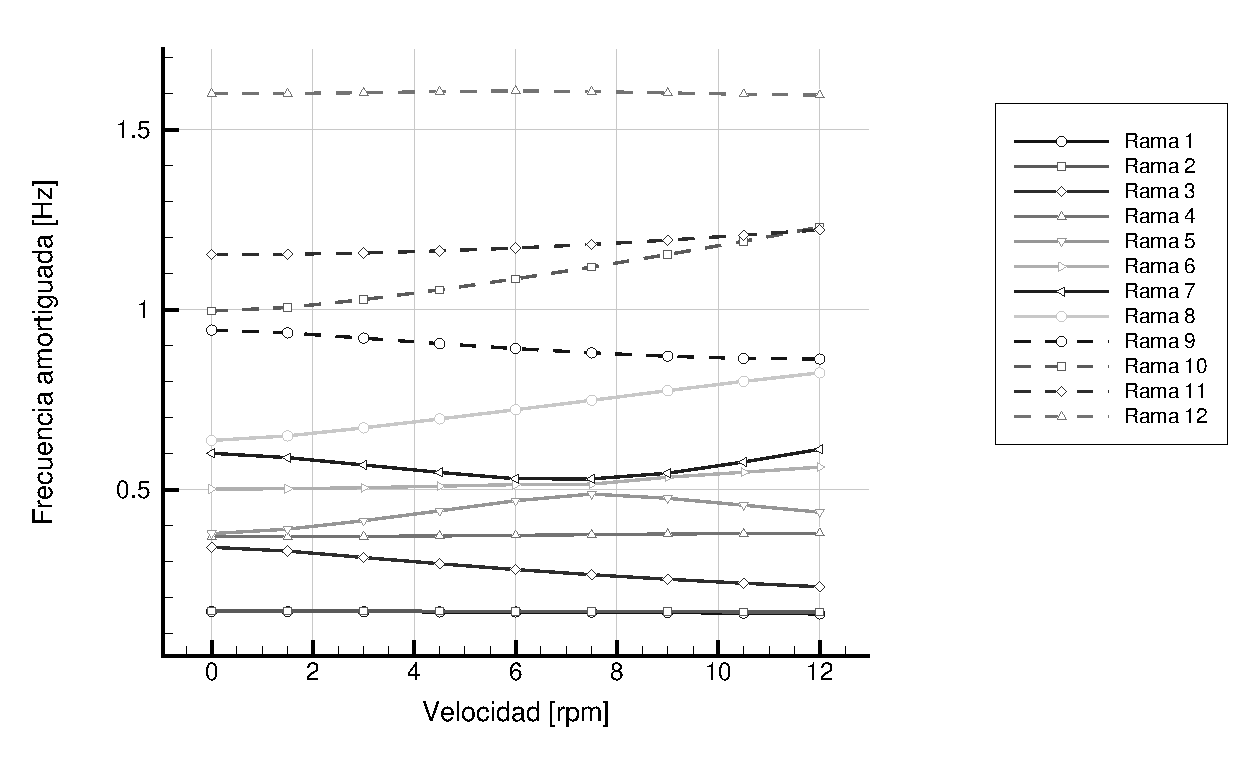
\includegraphics[width=\linewidth]{figures/tecplot/campbell.pdf}\end{minipage}
\par\medskip
\begin{minipage}{0.96\linewidth}\centering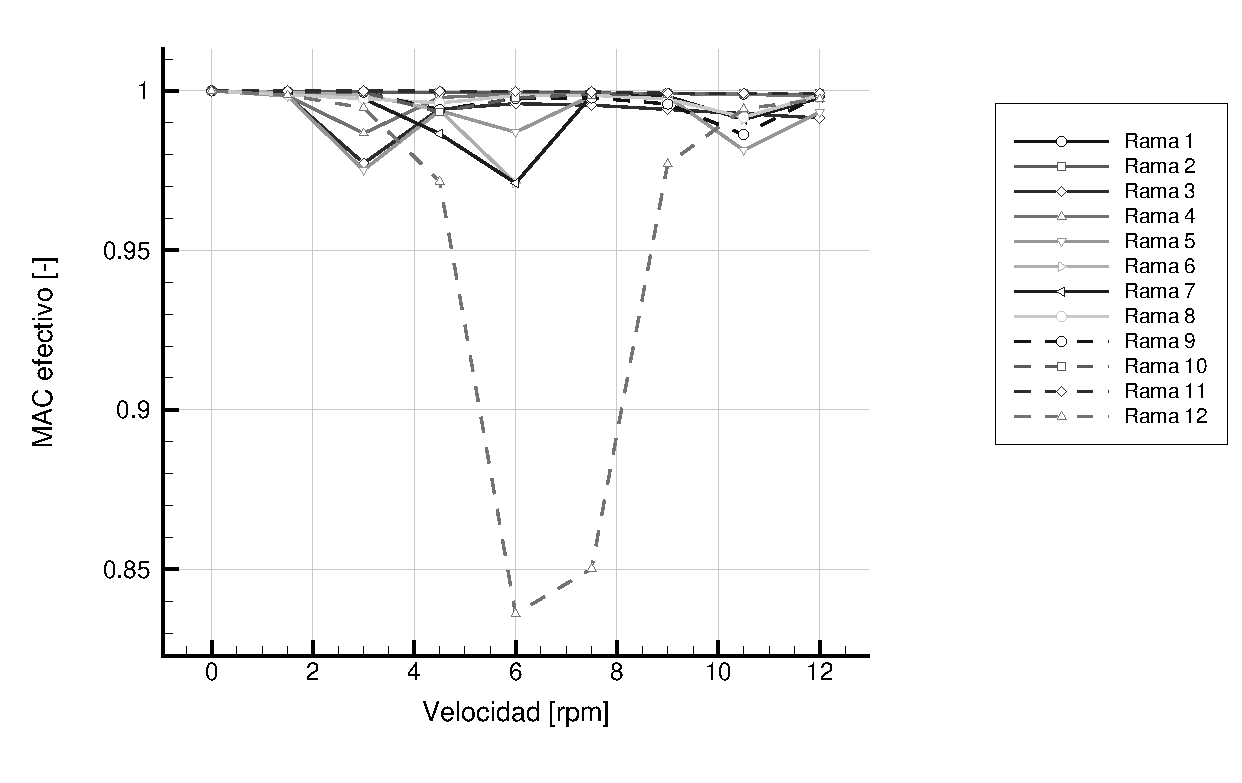
\includegraphics[width=\linewidth]{figures/tecplot/seguimiento_ramas.pdf}\end{minipage}
\caption{(a) Frecuencias amortiguadas del sistema congelado y (b) calidad efectiva del seguimiento por formas. Las líneas unen las velocidades calculadas; no constituyen modos de Floquet.}\label{fig:campbell-tecplot}
\end{figure}
\begin{figure}[htbp]\centering
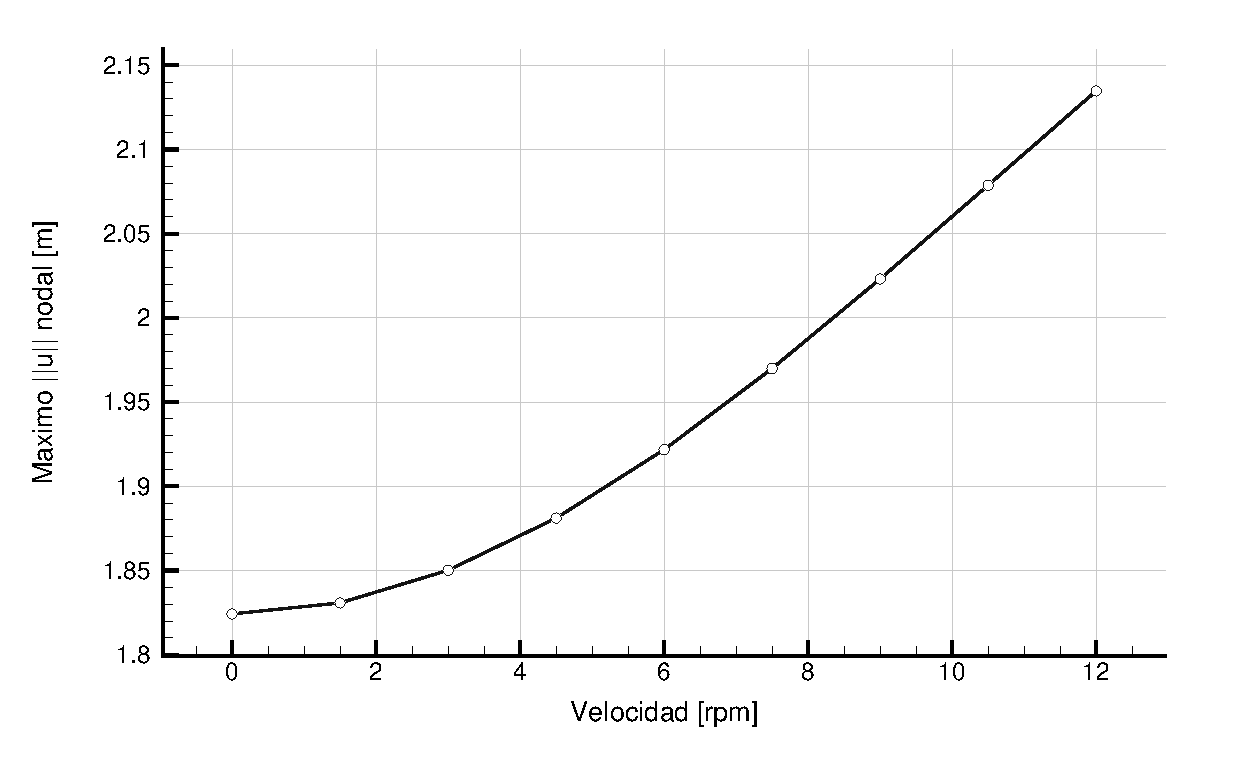
\includegraphics[width=.96\linewidth,height=.40\textheight,keepaspectratio]{figures/tecplot/equilibrio_velocidad.pdf}
\caption{Máxima norma de traslación nodal del equilibrio guardado frente a velocidad. Las líneas unen los estados almacenados.}\label{fig:equilibrio-tecplot}
\end{figure}
\begin{figure}[htbp]\centering
\begin{minipage}{0.96\linewidth}\centering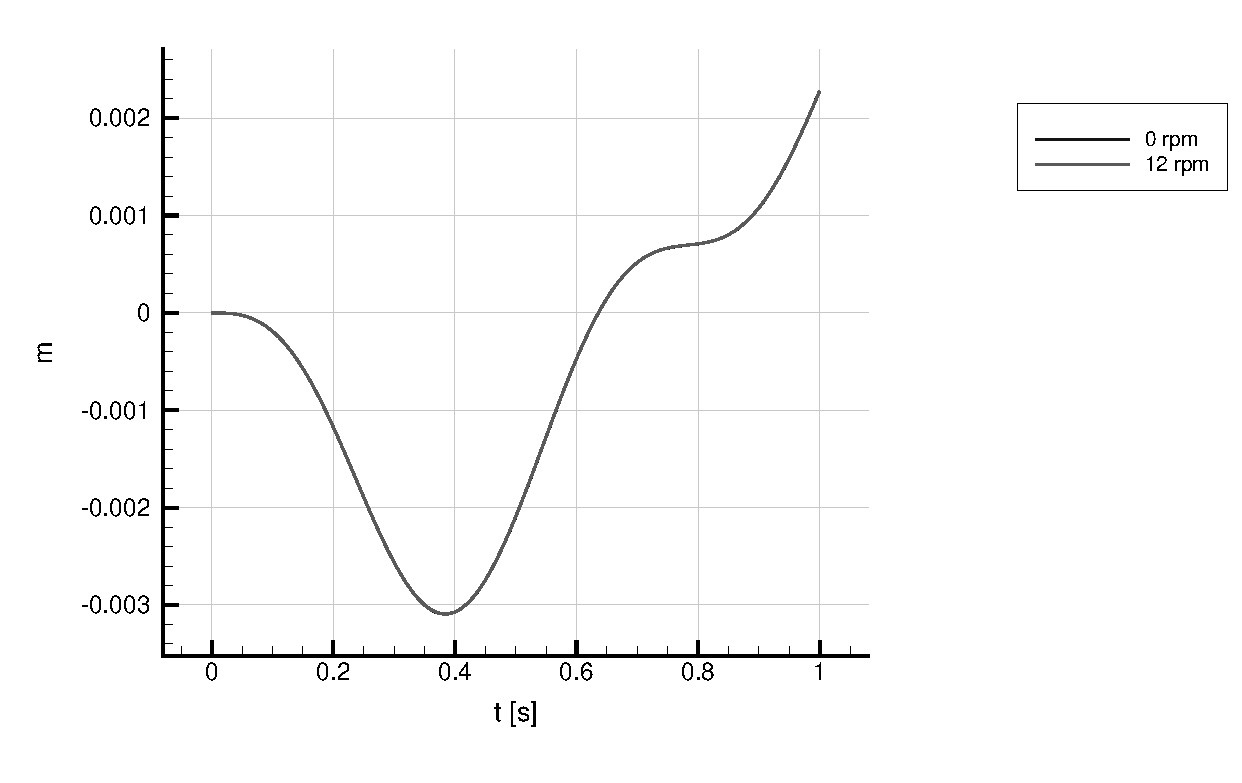
\includegraphics[width=\linewidth]{figures/tecplot/sismo_n129_ux.pdf}\end{minipage}
\par\medskip
\begin{minipage}{0.96\linewidth}\centering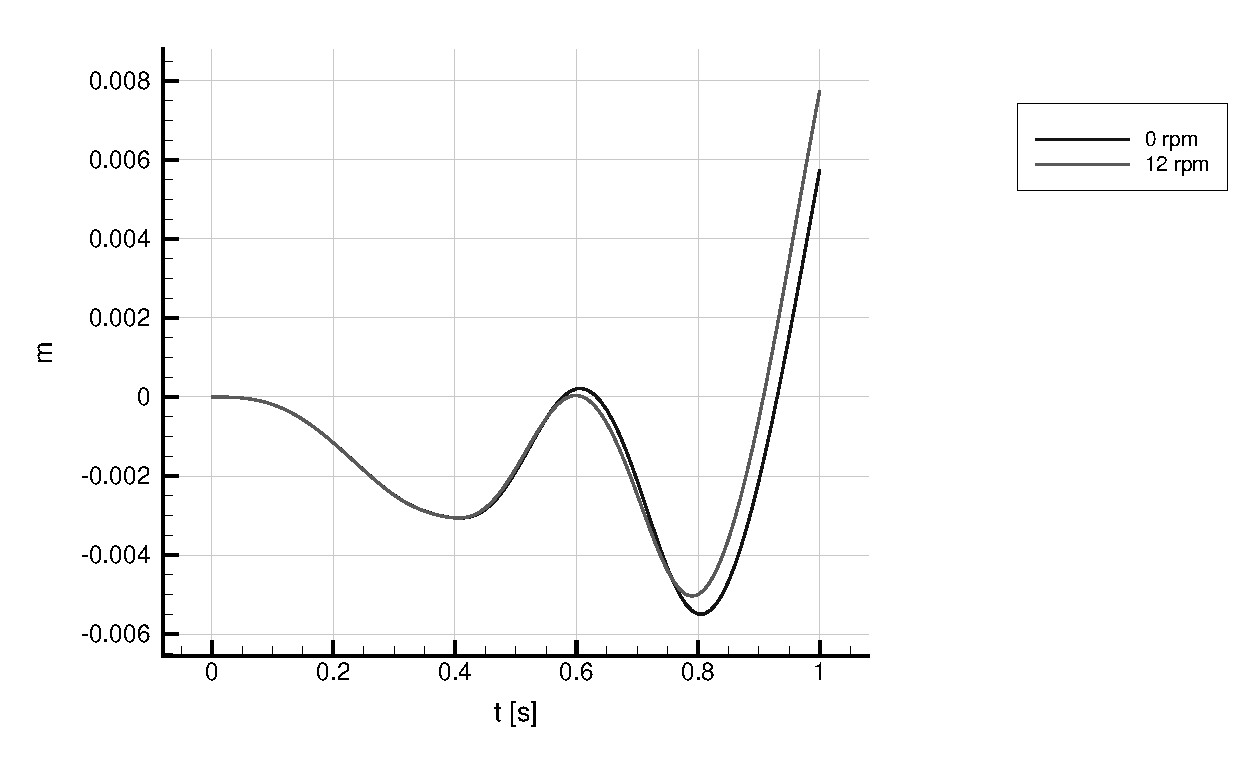
\includegraphics[width=\linewidth]{figures/tecplot/sismo_n56_ux.pdf}\end{minipage}
\caption{Perturbaciones de desplazamiento global X de (a) góndola, nodo 129, y (b) punta de pala 1, nodo 56, en los casos almacenados de 0 y 12 rpm. La ventana y el procesamiento corresponden al benchmark guardado; no se presenta un registro experimental adicional.}\label{fig:sismo-tecplot}
\end{figure}
\begin{figure}[htbp]\centering
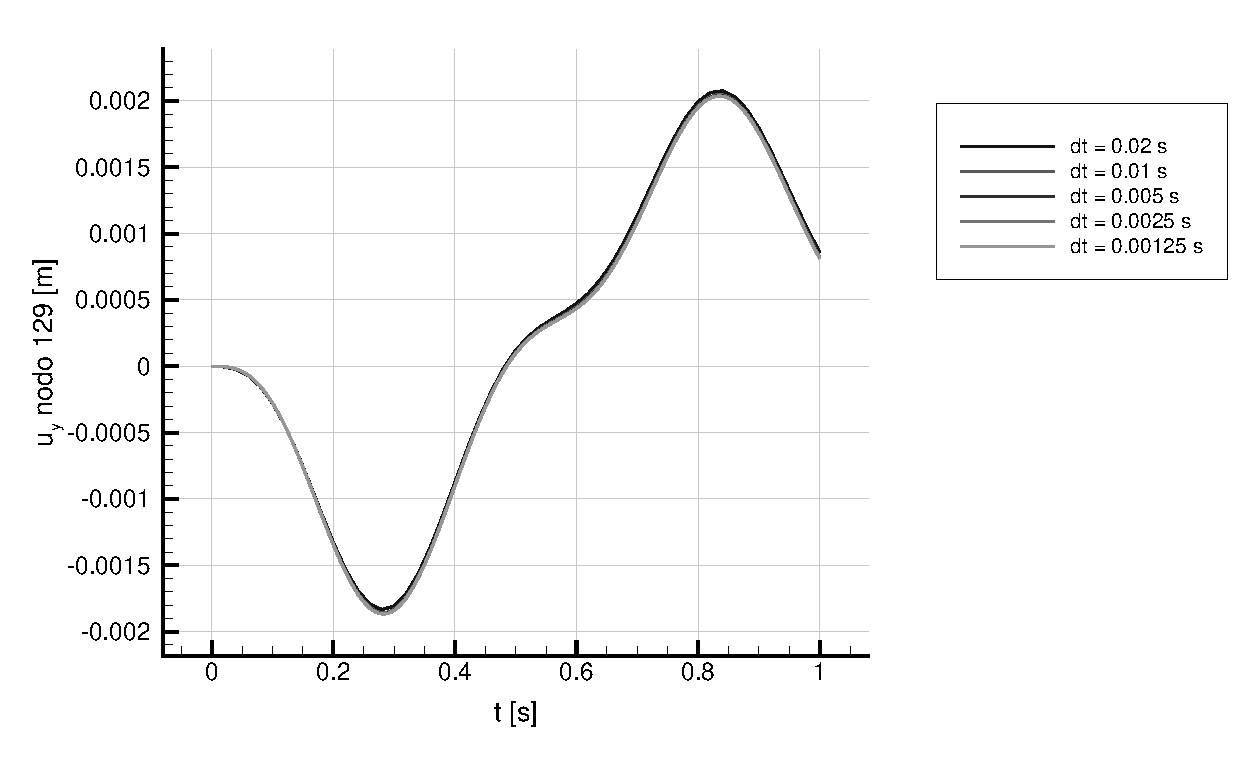
\includegraphics[width=.96\linewidth,height=.40\textheight,keepaspectratio]{figures/tecplot/sismo_convergencia.pdf}
\caption{Comparación temporal del desplazamiento global Y del nodo 129 para los cinco pasos almacenados. Se conserva la ventana de un segundo y la recuperación local de perturbaciones.}\label{fig:sismo-convergencia-tecplot}
\end{figure}
Las matrices y la reconstrucción física corresponden al mismo instante operativo. Las diferencias entre estados de giro incluyen equilibrio, transporte, restricciones temporales y transformación de coordenadas. No se atribuye el cambio de respuesta a un único bloque giroscópico aislado.
